\documentclass[a4paper, journal]{IEEEtran}
\usepackage[margin=0.75in]{geometry}
\IEEEoverridecommandlockouts
\usepackage{cite}
\usepackage{amsmath,amssymb,amsfonts}
\usepackage{algorithmic}
\usepackage{graphicx}
\usepackage{textcomp}
\usepackage{listings}
\usepackage{xcolor}
\usepackage{booktabs}
\usepackage{tikz}
\usepackage{times}
\usepackage{newtxmath}

\definecolor{codegreen}{rgb}{0,0.6,0}
\definecolor{codegray}{rgb}{0.5,0.5,0.5}
\definecolor{codepurple}{rgb}{0.58,0,0.82}
\definecolor{backcolour}{rgb}{0.95,0.95,0.92}

\lstset{
  language=Python,
  breaklines=true,
  breakatwhitespace=true,
  basicstyle=\ttfamily\footnotesize,
  keywordstyle=\color{codepurple},
  commentstyle=\color{codegreen},
  stringstyle=\color{red},
  captionpos=b,
  frame=single,
  showstringspaces=false,
  tabsize=4
}

\hyphenation{op-tical net-works semi-conduc-tor IEEE-Xplore}
\def\BibTeX{{\rm B\kern-.05em{\sc i\kern-.025em b}\kern-.08em
    T\kern-.1667em\lower.7ex\hbox{E}\kern-.125emX}}
\usepackage{balance}
\begin{document}

\title{Multilayer Perceptron Based Classifier for FashionMNIST Dataset using PyTorch}
\author{
    \IEEEauthorblockN{Dinanath Padhya\IEEEauthorrefmark{1}, Krishna Acharya\IEEEauthorrefmark{2}} \\
    \IEEEauthorblockA{\IEEEauthorrefmark{1}THA078BEI010 \quad \IEEEauthorrefmark{2}THA078BEI020\\
        Department of Electronics, Communication and Information Engineering\\
        Thapathali Campus, IOE, Tribhuvan University, Nepal\\
    }}

\maketitle

\begin{abstract}
    This study investigates the use of a Multilayer Perceptron (MLP) neural network for classifying images in the FashionMNIST dataset using PyTorch. The network was trained using normalized image data with an architecture of fully connected layers and ReLU activations. The experiment evaluates performance using metrics like accuracy, precision, recall, F1-score, and AUC-ROC. The results indicate that a simple MLP can achieve high performance for image classification tasks. ROC curves and training-validation loss plots were also generated to visualize model performance and convergence behavior.
\end{abstract}

\begin{IEEEkeywords}
    Multilayer Perceptron, FashionMNIST, PyTorch, Classification, Deep Learning, ROC Curve
\end{IEEEkeywords}

\section{Introduction}
\subsection{Literature Review}
Image classification is a central task in computer vision, where the goal is to assign predefined labels to input images. The introduction of deep learning has significantly advanced this field, with neural networks achieving remarkable accuracy across a wide range of image datasets. One such benchmark dataset is FashionMNIST, introduced by Xiao et al.~\cite{xiao2017fashion}, as a more realistic alternative to the original MNIST digit dataset created by LeCun et al.~\cite{lecun1998gradient}. FashionMNIST contains grayscale images of clothing items, offering increased complexity and diversity, thereby serving as a more effective benchmark for evaluating classification models.

Multilayer Perceptrons (MLPs), though simpler than Convolutional Neural Networks (CNNs), have proven to be effective in handling low-resolution image data~\cite{gu2018recent}. They offer a foundational understanding of neural network training dynamics and serve as a baseline for more advanced architectures. The theoretical principles behind deep learning, including optimization algorithms like Adam and activation functions such as ReLU, are extensively detailed by Goodfellow et al.~\cite{goodfellow2016deep}.

This experiment aims to develop an MLP using PyTorch and evaluate its performance on the FashionMNIST dataset using standard classification metrics. The study further analyzes model performance through ROC curves and loss plots to validate its generalization capability.


\subsection{Objectives}
This lab aims to design and evaluate a Multilayer Perceptron (MLP) using PyTorch to classify FashionMNIST images and analyze performance using standard metrics and visualization techniques.

\section{Mathematical Background}
\subsection{Activation Functions}
ReLU (Rectified Linear Unit) is used as the activation function. Defined as \( f(x) = \max(0, x) \), ReLU introduces non-linearity while avoiding vanishing gradient problems. The graph of the ReLU function is presented in Figure~\ref{fig:relu}.
\begin{figure}[h]
    \centering
    \begin{tikzpicture}[scale=1.2, axis/.style={very thick, ->, >=stealth}]
        % Axes
        \draw[axis] (-3,0) -- (3,0) node[right] {$x$};
        \draw[axis] (0,0) -- (0,3) node[above] {$f(x)$};
        % ReLU curve
        \draw[thick, green!60!black, domain=-3:0, samples=2] plot (\x,{0});
        \draw[thick, green!60!black, domain=0:3, samples=2] plot (\x,{\x});
        % Point of non-differentiability
        \filldraw[green!60!black] (0,0) circle (1.5pt);
        % Labels
        \node[left] at (0,0) {$0$};
    \end{tikzpicture}
    \caption{ReLU Activation Function: $f(x) = \max(0, x)$}
    \label{fig:relu}
\end{figure}
\subsection{Encoding}
Each grayscale image of size \(28 \times 28\) is flattened into a 784-dimensional vector. Labels are encoded as integers from 0 to 9 as shown in Table~\ref{tab:label_encoding}.
\begin{table}[h]
    \centering
    \caption{FashionMNIST Label Encoding}
    \label{tab:label_encoding}
    \begin{tabular}{ccll}
        \toprule
        \textbf{Label} & \textbf{Class Name} & \textbf{Label} & \textbf{Class Name} \\
        \midrule
        0              & T-shirt/top         & 1              & Trouser             \\
        2              & Pullover            & 3              & Dress               \\
        4              & Coat                & 5              & Sandal              \\
        6              & Shirt               & 7              & Sneaker             \\
        8              & Bag                 & 9              & Ankle boot          \\
        \bottomrule
    \end{tabular}
\end{table}


\subsection{Loss Functions}
Cross-Entropy Loss is used:
\begin{equation}
    \mathcal{L}(y, \hat{y}) = -\sum_{i} y_i \log(\hat{y}_i)
\end{equation}

This function measures the performance of classification models with softmax outputs.

\subsection{Optimizers}
Adam optimizer was used due to its ability to adapt learning rates during training, which enhances convergence.

\subsection{Training and Evaluation Loops}
Model training includes forward pass, loss calculation, backpropagation, and weight update. Validation loss is computed without weight updates. Evaluation is done on the test dataset.

\subsection{Dataset}
FashionMNIST is a labeled dataset of 60,000 training and 10,000 test grayscale images across 10 classes of fashion items. It is publicly available via torchvision.

% \section{Experiment \& Model Implementation}
% \subsection{Data Preprocessing}
% The image pixel values were normalized from their original range of $[0, 255]$ to $[-1, 1]$. The training and validation split was 90\% for training, 10\% for validation.

% \subsection{Model Architecture}
% The MLP consisted of:
% \begin{itemize}
%     \item Flatten layer (784 input)
%     \item Dense layer (128 units, ReLU)
%     \item Dense layer (64 units, ReLU)
%     \item Output layer (10 units, logits)
% \end{itemize}

% \subsection{Training Configuration}
% \begin{itemize}
%     \item Batch Size: 64 (training), 256 (validation/test)
%     \item Epochs: 10
%     \item Learning Rate: 0.001
%     \item Optimizer: Adam
%     \item Loss: CrossEntropy
% \end{itemize}

% \subsection{Evaluation Metrics}
% \begin{itemize}
%     \item Accuracy
%     \item Precision (macro)
%     \item Recall (macro)
%     \item F1-Score (macro)
%     \item ROC-AUC per class
% \end{itemize}

% \subsection{Code Snippet}
% \begin{lstlisting}[caption={Model Definition}]
% class MLP(nn.Module):
%     def __init__(self):
%         super(MLP, self).__init__()
%         self.model = nn.Sequential(
%             nn.Flatten(),
%             nn.Linear(784, 128),
%             nn.ReLU(),
%             nn.Linear(128, 64),
%             nn.ReLU(),
%             nn.Linear(64, 10)
%         )
%     def forward(self, x):
%         return self.model(x)
% \end{lstlisting}
\section{Experiment \& Model Implementation}

\subsection{Data Preprocessing}
Data preprocessing is a critical step in any machine learning pipeline, especially for image data. In this study, each $28 \times 28$ pixel grayscale image from the FashionMNIST dataset is first loaded as a two-dimensional array. To ensure consistent input distribution, the pixel values are normalized from their original range $[0, 255]$ to $[-1, 1]$ using the transformation $x' = (x / 127.5) - 1$. This normalization helps the network converge faster during training and prevents issues related to disparate value scales.

After normalization, the dataset is split into training, validation, and test subsets. 90\% of the original training data is used for training, and 10\% is reserved for validation to monitor overfitting and tune hyperparameters. The test set remains unseen throughout the training process and is used solely for final performance reporting.

\subsection{Model Architecture}
The architecture designed for this experiment is a fully connected Multilayer Perceptron (MLP) with two hidden layers. The choice of architecture is influenced by the relatively low spatial resolution of FashionMNIST images, which allows a dense network to capture meaningful patterns without the spatial inductive biases of convolutional layers.

The architecture is as follows:
\begin{itemize}
    \item \textbf{Input Layer:} Flattens the $28 \times 28$ image into a 784-dimensional feature vector.
    \item \textbf{First Hidden Layer:} Fully connected (Linear) layer with 128 neurons, followed by a ReLU activation function. This layer projects the input into a higher-dimensional space, allowing the network to learn complex feature representations.
    \item \textbf{Second Hidden Layer:} Another fully connected layer with 64 neurons and ReLU activation. This intermediate compression helps in extracting higher-level features while preventing overfitting due to excessive network width.
    \item \textbf{Output Layer:} A dense layer with 10 output neurons, corresponding to the 10 clothing categories. The output logits are used in combination with the cross-entropy loss during training.
\end{itemize}

\subsection{Training Pipeline and Hyperparameters}
The network is implemented and trained in PyTorch. Key hyperparameters and configurations are:
\begin{itemize}
    \item \textbf{Batch Size:} 64 for training, 256 for validation and test. Smaller batch sizes during training enable more frequent updates and potentially better generalization.
    \item \textbf{Epochs:} 10 full passes over the training, and 10 epochs were sufficient to ensure convergence without overfitting.
    \item \textbf{Learning Rate:} 0.001, chosen as a standard starting point for Adam optimizer and further validated via loss curve smoothness.
    \item \textbf{Optimizer:} Adam, a variant of stochastic gradient descent that adaptively scales learning rates per parameter, resulting in robust and efficient convergence.
    \item \textbf{Loss Function:} Cross-entropy loss, suitable for multi-class classification with mutually exclusive categories.
\end{itemize}

During each training epoch, the model undergoes a forward pass to compute predictions, calculates the loss, performs backpropagation to compute gradients, and updates weights. Validation loss and metrics are computed after each epoch to track generalization performance and detect overfitting.


\subsection{Evaluation Metrics}
Evaluating classification models requires a comprehensive suite of metrics, especially for multi-class datasets such as FashionMNIST. The following metrics were employed:

\begin{itemize}
    \item \textbf{Accuracy:} The fraction of correct predictions among all predictions, defined as
          \[
              \text{Accuracy} = \frac{\text{Number of Correct Predictions}}{\text{Total Predictions}}
          \]
          While intuitive, accuracy alone may not suffice in imbalanced datasets.

    \item \textbf{Precision ~:} Measures the proportion of positive identifications that were actually correct. For multi-class tasks, it is the arithmetic mean of precision values for all classes:
          \[
              \text{Precision}_\text{} = \frac{1}{K} \sum_{i=1}^{K} \frac{\text{TP}_i}{\text{TP}_i + \text{FP}_i}
          \]
          where $K$ is the number of classes, $\text{TP}_i$ is true positives for class $i$, and $\text{FP}_i$ is false positives for class $i$.

    \item \textbf{Recall ~:} Measures the proportion of actual positives that were identified correctly:
          \[
              \text{Recall}_\text{} = \frac{1}{K} \sum_{i=1}^{K} \frac{\text{TP}_i}{\text{TP}_i + \text{FN}_i}
          \]
          where $\text{FN}_i$ is false negatives for class $i$.

    \item \textbf{F1-score ~:} The harmonic mean of precision and recall, providing a balanced assessment in case of class imbalance:
          \[
              \text{F1}_\text{} = \frac{1}{K} \sum_{i=1}^{K} 2 \cdot \frac{\text{Precision}_i \cdot \text{Recall}_i}{\text{Precision}_i + \text{Recall}_i}
          \]

    \item \textbf{ROC-AUC (Receiver Operating Characteristic – Area Under Curve):} For each class, a one-vs-rest strategy is used to compute the ROC curve, which plots the true positive rate against the false positive rate at various threshold settings. The AUC summarizes the classifier's ability to distinguish between classes; a higher value indicates better performance.
\end{itemize}

This comprehensive metric set ensures robust evaluation by considering not just overall correctness, but also the quality of predictions per class, and the trade-off between precision and recall. The ROC-AUC further visualizes separability and potential performance under different operating thresholds.

\subsection{Code Snippet}
Below is the core implementation of the MLP in PyTorch:

\begin{lstlisting}[caption={Model Definition}]
class MLP(nn.Module):
    def __init__(self):
        super(MLP, self).__init__()
        self.model = nn.Sequential(
            nn.Flatten(),
            nn.Linear(784, 128),
            nn.ReLU(),
            nn.Linear(128, 64),
            nn.ReLU(),
            nn.Linear(64, 10)
        )
    def forward(self, x):
        return self.model(x)
\end{lstlisting}

\subsection{Training Procedure and Monitoring}
Training and validation losses are tracked at each epoch. The model's performance is periodically assessed on the validation set. If the validation loss ceases to improve, this may indicate overfitting, and training is terminated early

Visualizations such as loss curves (training vs validation) and ROC curves for each class provide insights into convergence behavior and class separability, respectively.


\section{Result}
The model achieved the following performance on the test dataset:

\begin{table}[h]
    \centering
    \caption{Performance Metrics}
    \begin{tabular}{lc}
        \toprule
        Metric    & Value  \\
        \midrule
        Accuracy  & 0.8829 \\
        Precision & 0.8821 \\
        Recall    & 0.8829 \\
        F1-Score  & 0.8822 \\
        \bottomrule
    \end{tabular}
\end{table}

\subsection{ROC Curves}
The ROC-AUC was computed for each class using a one-vs-rest approach. The plotted curves indicate high separability between classes. The lowest separability was observed for the class 6 (shirt), with an AUC of 0.96, while the highest was for class 1 (Trouser), with an AUC of 1.

\begin{figure}[h]
    \centering
    \includegraphics[width=0.45\textwidth]{img/lab3/roc_curves_all_classes.pdf}
    \caption{ROC Curves for All Classes}
\end{figure}

\subsection{Training vs Validation Loss}
Loss curves indicate smooth convergence without signs of overfitting.

\begin{figure}[h]
    \centering
    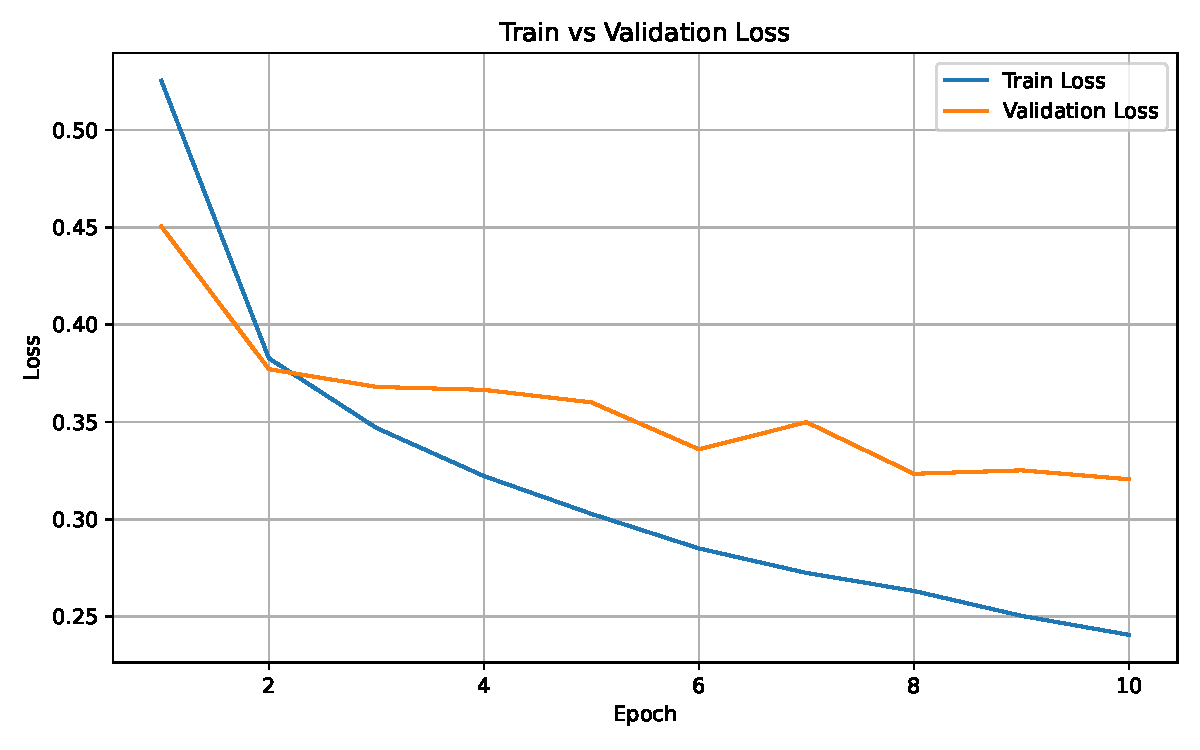
\includegraphics[width=0.5\textwidth]{img/lab3/train_vs_val_loss.pdf}
    \caption{Training vs Validation Loss}
\end{figure}

\section{Conclusion}
This experiment validates that a simple Multilayer Perceptron can classify FashionMNIST images with high accuracy and generalization capability. The ROC and loss plots further support the model’s robustness.


\balance
\bibliographystyle{IEEEtran}
\bibliography{ref}

\end{document}
